SyVOLT has a number of unique features, outlined below.

\subsection{Input Independence and Exhaustiveness} 

SyVOLT proves that pre-/post-condition contracts hold for a model transformation.
Such contracts establish relations between patterns occurring in input and output
models of a model transformation. If a contract holds, a formal guarantee
exists that whenever a transformation's input model contains the pattern
specified in the pre-condition of the contract, the transformation's output model will contain
the pattern specified in the contract's post-condition. Contracts can 
optionally include traceability relations between input and output patterns. 
Our technique is exhaustive and input-independent, in the sense that whenever a contract holds, it
will hold for all possible input models for that transformation. This is possible
because SyVOLT operates on specifications of out-place model transformations,
where unbounded loops and model element deletions are not allowed. A discussion
on the soundness and completeness of our approach is provided
in~\cite{Lucio2014}.

%SyVOLT proves
%contracts in an input-independent manner, relying only on the specification of the
%transformation.



\subsection{Integration with Eclipse / Graphical Modelling}

Eclipse is a popular development environment, as many model transformation tools
such as ATL, DSLTrans~\cite{Barroca2011} and
EGL~\cite{eglTool} are integrated with the Eclipse
Modeling Framework (EMF)~\cite{emfTool}. To take
advantage of this ecosystem, SyVOLT integrates with EMF to represent models in a
multitude of syntaxes, from graphical to textual. Modellers may then operate
in their preferred syntax, although the authors suggest the visual
representation of a contract in the SyVOLT editor allows for intuitive
understanding of the contract's meaning.

%\subsection{Graphical Modelling of Model Transformation Contracts}



%If a textual (logical or mathematical) editor where to be used, the user would
%need an extra system of identifiers to correctly prescribe the associations
% between pre and post-condition elements whereas in the visual representation, the user graphically builds the associations between those elements.
%\levi{Claudio, I don't understand this sentence}
%\cgg{Please tell me now if you can understand it.}

%The visual representation of a contract has all the necessary information to
% derive the correct logical expression to be used by the internal SyVolt prover.

\begin{figure}
%\centering
%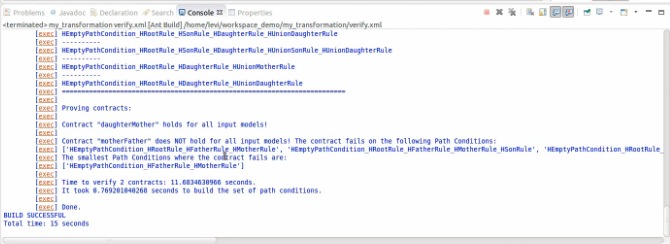
\includegraphics[width=0.5\textwidth]{figures/output}

\scriptsize
\tt
> Proving contracts:

> Contract ``daughterMother'' holds for all input models!
\\
> Contract ``motherFather'' does NOT hold for all input models! The contract
fails on the following Path Conditions:
[`EmptyPathCondition\_RootRule\_FatherRule\_MotherRule', ...]

> The smallest Path Conditions where the contract fails are:
[`EmptyPathCondition\_FatherRule\_MotherRule']
\\
> Time to verify 2 contracts: 11.6834638966 seconds.
%It took 0.769201040268 seconds to build the set of path conditions.
\caption{Sample output of the contract prover}
\label{fig:output}
\vspace{-.5cm}
\end{figure}

\subsection{Push-Button Proofs}
\label{sec:push_button_proofs}
The proving process for a SyVOLT contract is fully automatic and all of the
approach's formal details are completely hidden from the user. Once the
transformation and the contracts of interest are created, one command will start
the property proving process. This process will automatically create all
required artifacts (as detailed in Section~\ref{sec:arch}), run the process, and
provide the results to the user within the Eclipse environment. This allows the user to continually stay within the
Eclipse environment, where he or she develops the contracts and the
model transformations.

%Figure~\ref{fig:output} shows an example of the output presented to the user, detailing which contracts hold and do not hold.

\subsection{Counter-Examples}

When a given contract does not hold on a given model transformation,
SyVOLT can produce additional information for the user to pinpoint where
the contract's violation occurs. This information is in
the form of the set of model transformation rules used to build a particular
path condition for which the contract fails. A counter-example is any input model where this set of rules would execute. For example, the sample output in Figure~\ref{fig:output} alerts the user that the contract \textit{motherFather} will fail when only the \textit{mother} and \textit{father} rules execute in the transformation.

\subsection{Based on Symbolic Execution}

Our technique shares its principles with symbolic execution, a classic method to
verify code. The underlying idea entails building a finite representation of the
(infinite) set of computations that can be expressed by a model transformation
specification. In this context, each symbolic execution -- which in the context
of our work we call a \emph{path condition} -- is an overlapping combination
of a subset of the transformation's rules. Because a path condition contains a
number of rules, it represents the execution of the model transformation over any input model those rules match on.


Contracts of interest are proved on the set of path conditions built for a
model transformation, and are extrapolated to the infinite set of
the model transformation's computations through an abstraction
relation~\cite{Lucio2014}.

% Our model transformation verification technique relies on models as the
% means to internally represent both symbolic executions and contracts. SyVOLT
% then reasons over these graphs to build a proof that contracts hold or do not
% hold.

% Note that by using a typed graph representation, our technique can prove
% contracts that include constraints on the structure and the attributes of the
% input and output models. 

% \levi{keep the text from here on?} An example of this would be in the
% Families-To-Persons transformation from the ATL zoo [CITE]. In this transformation, the name for a person in the
% output graph is a concatenation of two strings \cgg{instead of ''strings``,
% should be ''attributes``} from elements in the input graph. Our contract prover
% can prove that this concatenation will be valid in all cases.

\subsection{Proving Contracts about ATL Model Transformations}
The Atlas Transformation Language (ATL)~\cite{atlTool} is
commonly-used in both industrial and academic applications. In order to enable contract proving on ATL transformations, we
have developed a higher-order transformation that is able to automatically
transform declarative ATL transformations into DSLTrans transformations~\cite{Oakes}. 
In the future we will integrate this higher-order transformation into SyVOLT's
user interface.

\subsection{Scalability and Speed}

We have some evidence that SyVOLT scales to transformations of practical
interest. In particular we have verified contracts on DSLTrans transformations with up to
over 60 rules, and ATL transformations with up to 13 rules~\cite{Oakes}. From our own
experience, the size of a DSLTrans transformation ranges from 10 up to 50 rules, while the average size of an ATL
transformation is around 20 rules~\cite{KuselSWRSK13}.
Even though our technique is exhaustive, our experiments show that verification can be performed within seconds.
Gehan Selim's PhD thesis~\cite{Selim2015} provides further evidence of SyVOLT's speed, by verifying a relatively large model transformation
for giving semantics to the UML-RT language in terms of the Kiltera process
language~\cite{PosseDingel2014}. SyVOLT's symbolic execution engine is fully
homegrown~\cite{LucioVang} and does not depend on third-party solvers. Although
this has implied a large effort to build the codebase, it has allowed us to
have the required control over the code to iteratively optimize the engine for
space and time economy.
\cite{Selim2014} demonstrates that our prover is substantially faster than
similar approaches based on SAT solvers.




%  This means that any input model that belongs to the family of the
% counter-example - i.e., fits the description given by the contract proving
% process - causes the model transformation to violate the contract.
% We suggest that this supports a transformation
% development method analogous to 'test-driven development'. In this method,
% development would be routinely punctuated by contract proof in order to catch
% errors early and store test cases - the counter examples produced - to be used
% in the future.




%, and this makes the interaction with SyVOLT easier since the modeler
%can use the model editor that he/she finds most convenient.
%Internally, SyVOLT uses the Himesis format~\cite{Provost2006} to represent
% models.

%\subsection{Model Driven Developed GUI\levi{this text is subsumed by section
%III a)}}
%\label{sec:mdd_gui}

%To take advantage of the productivity promised by MDD, we used a language
% called Eugenia[CITE] to develop the SyVolt contract editor shown in
%Figure~\ref{fig:eclipse_frontend}.
%With this approach, the SyVolt editor was developed in about 4 man-hours.





 